%%%%%%%%%%%%%%%%%%%%%%%%%%%%%%%%%%%%%%%%%%%%%%%%%%%%%%%%%%%%%%%%%%%%%%%%%%%%%%%%
\chapter{Working on graphs without properties}
\label{sec:Working-on-graphs-without-properties}
%%%%%%%%%%%%%%%%%%%%%%%%%%%%%%%%%%%%%%%%%%%%%%%%%%%%%%%%%%%%%%%%%%%%%%%%%%%%%%%%

Now that we can build a graph, there are some things we can do.

\begin{itemize}
  \item
    Getting the vertices' out degrees: 
    see chapter \ref{subsec:get_vertex_out_degrees}
  \item
    Create a direct-neighbour subgraph from a vertex descriptor
  \item
    Create all direct-neighbour subgraphs from a graphs
  \item
    Saving a graph without properties to .dot file: 
    see chapter \ref{subsec:save_graph_to_dot}
  \item
    Loading an undirected graph without properties from .dot file: 
    see chapter \ref{subsec:load_undirected_graph_from_dot}
  \item
    Loading a directed graph without properties from .dot file: 
    see chapter \ref{subsec:load_directed_graph_from_dot}
\end{itemize}


%%%%%%%%%%%%%%%%%%%%%%%%%%%%%%%%%%%%%%%%%%%%%%%%%%%%%%%%%%%%%%%%%%%%%%%%%%%%%%%%
\section{Getting the vertices' out degree}
\label{subsec:get_vertex_out_degrees}
%%%%%%%%%%%%%%%%%%%%%%%%%%%%%%%%%%%%%%%%%%%%%%%%%%%%%%%%%%%%%%%%%%%%%%%%%%%%%%%%

Let's measure the out degree of all vertices in a graph! 

The out degree of a vertex is the number of edges that originate at it.

The number of connections is called the \verb;degree; of the vertex.
There are three types of degrees:

\begin{itemize}
  \item in degree: the number of incoming connections, 
    using \verb;in_degree; \index{in\_degree}
    (not \verb;boost::in_degree; \index{boost::in\_degree does not exist} )
  \item out degree: the number of outgoing connections, 
    using \verb;out_degree; \index{out\_degree}
    (not \verb;boost::out_degree; \index{boost::out\_degree does not exist})
  \item degree: sum of the in degree and out degree, 
    using \verb;degree; \index{degree}
    (not \verb;boost::degree; \index{boost::degree does not exist})
\end{itemize}

Listing \ref{lst:get_vertex_out_degrees}
shows how to obtain these:

\lstinputlisting[
  caption = Get the vertices' out degrees,
  label = lst:get_vertex_out_degrees
]{get_vertex_out_degrees.impl}
\index{Get vertex out degrees}

The structure of this algorithm is similar to 
\verb;get_vertex_descriptors; (algorithm \ref{lst:get_vertex_descriptors}), 
except that the out degrees from the vertex descriptors are stored.
The out degree of a vertex iterator is obtained from 
the function \verb;out_degree; \index{out\_degree}
(not boost::out\_degree \index{boost::out\_degree does not exist}!).
 
Albeit that the $K_{2}$
graph and the two-state Markov chain are rather simple, we can use it to
demonstrate \verb;get_vertex_out_degrees; on, as shown in algorithm 
\ref{lst:get_vertex_out_degrees_demo}.

\lstinputlisting[
  caption = Demonstration of the get\_vertex\_out\_degrees function,
  label = lst:get_vertex_out_degrees_demo
]{get_vertex_out_degrees_demo.impl}

It is expected that $K_{2}$
has one out-degree for every vertex, where the two-state Markov chain is
expected to have two out-degrees per vertex.

%%%%%%%%%%%%%%%%%%%%%%%%%%%%%%%%%%%%%%%%%%%%%%%%%%%%%%%%%%%%%%%%%%%%%%%%%%%%%%%%
\section{$\triangle$ Is there an edge between two vertices?}
\label{subsec:has_edge_between_vertices}
%%%%%%%%%%%%%%%%%%%%%%%%%%%%%%%%%%%%%%%%%%%%%%%%%%%%%%%%%%%%%%%%%%%%%%%%%%%%%%%%

If you have two vertex descriptors, you can check if these are connected
 by an edge:

\lstinputlisting[
  caption = Check if there exists an edge between two vertices,
  label = lst:has_edge_between_vertices
]{has_edge_between_vertices.impl}
\index{Has edge between vertices}

This code uses the function \verb;edge; \index{edge}
(not boost::edge \index{boost::edge does not exist}): 
it returns a pair consisting of an edge descriptor and a boolean indicating
if it is a valid edge descriptor.
The boolean will be true if there exists an edge between the two vertices
and false if not.

The demo shows that there is an edge between the two vertices of a 
$K_{2}$ graph, but there are no self-loops (edges that original and end at the
 same vertex).

\lstinputlisting[
  caption = Demonstration of the has\_edge\_between\_vertices function,
  label = lst:has_edge_between_vertices_demo
]{has_edge_between_vertices_demo.impl}

%%%%%%%%%%%%%%%%%%%%%%%%%%%%%%%%%%%%%%%%%%%%%%%%%%%%%%%%%%%%%%%%%%%%%%%%%%%%%%%%
\section{$\triangle$ Get the edge between two vertices}
\label{subsec:get_edge_between_vertices}
%%%%%%%%%%%%%%%%%%%%%%%%%%%%%%%%%%%%%%%%%%%%%%%%%%%%%%%%%%%%%%%%%%%%%%%%%%%%%%%%

If you have two vertex descriptors, you can use these to find the edge between
them.

\lstinputlisting[
  caption = Get the edge between two vertices,
  label = lst:get_edge_between_vertices
]{get_edge_between_vertices.impl}
\index{Get edge between vertices}

This code does assume that there is an edge between the two vertices.

The demo shows how to get the edge between two vertices, deleting it, and
 checking for success.

\lstinputlisting[
  caption = Demonstration of the get\_edge\_between\_vertices function,
  label = lst:get_edge_between_vertices_demo
]{get_edge_between_vertices_demo.impl}

%%%%%%%%%%%%%%%%%%%%%%%%%%%%%%%%%%%%%%%%%%%%%%%%%%%%%%%%%%%%%%%%%%%%%%%%%%%%%%%%
\section{$\triangle$$\triangle$ Create a direct-neighbour subgraph from a vertex descriptor}
\label{subsec:create_direct_neighbour_subgraph}
%%%%%%%%%%%%%%%%%%%%%%%%%%%%%%%%%%%%%%%%%%%%%%%%%%%%%%%%%%%%%%%%%%%%%%%%%%%%%%%%

Suppose you have a vertex of interest its vertex descriptor.
Let's say you want to get a subgraph of that vertex and its direct neighbours
only.
This means that all vertices of that subgraph are adjacent vertices and
that the edges go either from focal vertex to its neighbours, or from adjacent
vertex to adjacent neighbour.

Here is the \verb;create_direct_neighbour_subgraph; code:

\lstinputlisting[
  caption = Get the direct-neighbour subgraph from a vertex descriptor,
  label = lst:create_direct_neighbour_subgraph
]{create_direct_neighbour_subgraph.impl}
\index{Create direct-neighbour subgraph}

This demonstration code shows that the direct-neighbour graph of each vertex
 of a $K_{2}$ graphs is ... a $K_{2}$ graph!

\lstinputlisting[
  caption = Demo of the create\_direct\_neighbour\_subgraph function,
  label = lst:create_direct_neighbour_subgraph_demo
]{create_direct_neighbour_subgraph_demo.impl}

Note that this algorithm works on both undirected and directional graphs.
If the graph is directional, only the out edges will be copied.
To also copy the vertices connected with inward edges, use 
\ref{subsec:create_direct_neighbour_subgraph_including_in_edges}

%%%%%%%%%%%%%%%%%%%%%%%%%%%%%%%%%%%%%%%%%%%%%%%%%%%%%%%%%%%%%%%%%%%%%%%%%%%%%%%%
\section{$\triangle$$\triangle$ Create a direct-neighbour subgraph from a vertex descriptor including inward edges}
\label{subsec:create_direct_neighbour_subgraph_including_in_edges}
%%%%%%%%%%%%%%%%%%%%%%%%%%%%%%%%%%%%%%%%%%%%%%%%%%%%%%%%%%%%%%%%%%%%%%%%%%%%%%%%

Too bad, this algorithm does not work yet.

\lstinputlisting[
  caption = Get the direct-neighbour subgraph from a vertex descriptor,
  label = lst:create_direct_neighbour_subgraph_including_in_edges
]{create_direct_neighbour_subgraph_including_in_edges.impl}
\index{Create direct-neighbour subgraph\_including\_in\_edges}

%%%%%%%%%%%%%%%%%%%%%%%%%%%%%%%%%%%%%%%%%%%%%%%%%%%%%%%%%%%%%%%%%%%%%%%%%%%%%%%%
\section{$\triangle$$\triangle$ Creating all direct-neighbour subgraphs from a graph without properties}
\label{subsec:create_all_direct_neighbour_subgraphs}
%%%%%%%%%%%%%%%%%%%%%%%%%%%%%%%%%%%%%%%%%%%%%%%%%%%%%%%%%%%%%%%%%%%%%%%%%%%%%%%%

Using the previous function, it is easy to create all direct-neighbour subgraphs
 from a graph without properties:

\lstinputlisting[
  caption = Create all direct-neighbour subgraphs from a graph without properties,
  label = lst:create_all_direct_neighbour_subgraphs
]{create_all_direct_neighbour_subgraphs.impl}
\index{Create all direct-neighbour subgraphs}

This demonstration code shows that all two direct-neighbour graphs 
of a $K_{2}$ graphs are ... $K_{2}$ graphs!

\lstinputlisting[
  caption = Demo of the create\_all\_direct\_neighbour\_subgraphs function,
  label = lst:create_all_direct_neighbour_subgraphs_demo
]{create_all_direct_neighbour_subgraphs_demo.impl}

%%%%%%%%%%%%%%%%%%%%%%%%%%%%%%%%%%%%%%%%%%%%%%%%%%%%%%%%%%%%%%%%%%%%%%%%%%%%%%%%
\subsection{$\triangle$ Are two graphs isomorphic?}
\label{subsec:is_isomorphic}
%%%%%%%%%%%%%%%%%%%%%%%%%%%%%%%%%%%%%%%%%%%%%%%%%%%%%%%%%%%%%%%%%%%%%%%%%%%%%%%%

You may want to check if two graphs are isomorphic.
 That is: if they have the same shape.

\lstinputlisting[
  caption = Check if two graphs are isomorphic,
  label = lst:is_isomorphic
]{is_isomorphic.impl}
\index{Is isomorphic}

This demonstration code shows that a 
$K_{3}$ graph is not equivalent to a 3-vertices path graph:

\lstinputlisting[
  caption = Demo of the is\_isomorphic function,
  label = lst:is_isomorphic_demo
]{is_isomorphic_demo.impl}

%%%%%%%%%%%%%%%%%%%%%%%%%%%%%%%%%%%%%%%%%%%%%%%%%%%%%%%%%%%%%%%%%%%%%%%%%%%%%%%%
\section{$\triangle$$\triangle$ Count the number of connected components in an directed graph}
\label{subsec:count_directed_graph_connected_components}
%%%%%%%%%%%%%%%%%%%%%%%%%%%%%%%%%%%%%%%%%%%%%%%%%%%%%%%%%%%%%%%%%%%%%%%%%%%%%%%%

A directed graph may consist out of two components, that are connected within
each, but unconnected between them.
Take for example, a graph of two isolated edges, with four vertices.

\begin{figure}
  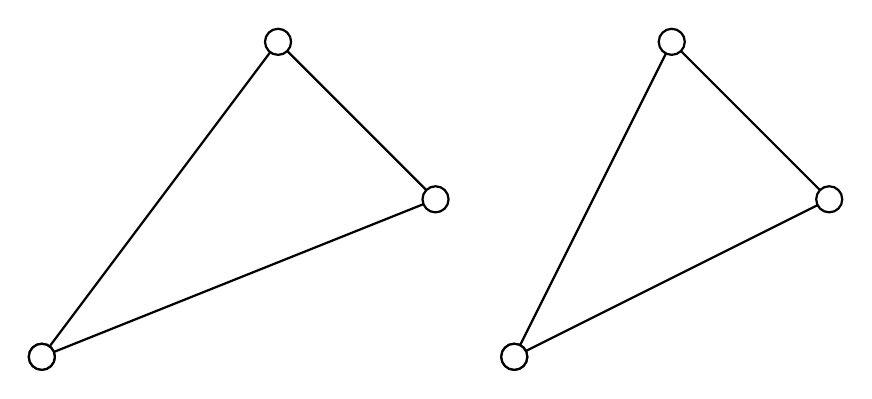
\begin{tikzpicture}
    \draw[thick] 
    (0,0) node[draw=black,fill=white,shape=circle,text=white] {} 
      -> (5,2) node[draw=black,fill=white,shape=circle,text=white] {} 
      -> (3,4) node[draw=black,fill=white,shape=circle,text=white] {} 
      -> (0,0) node[draw=black,fill=white,shape=circle,text=white] {} 
    (6,0) node[draw=black,fill=white,shape=circle,text=white] {} 
      -> (10,2) node[draw=black,fill=white,shape=circle,text=white] {} 
      -> (8,4) node[draw=black,fill=white,shape=circle,text=white] {} 
      -> (6,0) node[draw=black,fill=white,shape=circle,text=white] {} 
    ;
  \end{tikzpicture}
  \caption{Example of a directed graph with two components}
  \label{fig:count_directed_graph_connected_components}
\end{figure}

This algorithm counts the number of connected components:

\lstinputlisting[
  caption = Count the number of connected components,
  label = lst:count_directed_graph_connected_components
]{count_directed_graph_connected_components.impl}
\index{Count connected components}

The complexity of this algorithm is 
$O(\left|V\right|+\left|E\right|)$.

This demonstration code shows that two solitary edges are correctly counted
as being two components:

\lstinputlisting[
  caption = Demo of the count\_directed\_graph\_connected\_components function,
  label = lst:count_directed_graph_connected_components_demo
]{count_directed_graph_connected_components_demo.impl}

%%%%%%%%%%%%%%%%%%%%%%%%%%%%%%%%%%%%%%%%%%%%%%%%%%%%%%%%%%%%%%%%%%%%%%%%%%%%%%%%
\section{$\triangle$$\triangle$ Count the number of connected components in an undirected graph}
\label{subsec:count_undirected_graph_connected_components}
%%%%%%%%%%%%%%%%%%%%%%%%%%%%%%%%%%%%%%%%%%%%%%%%%%%%%%%%%%%%%%%%%%%%%%%%%%%%%%%%

An undirected graph may consist out of two components, that are connect
within each, but unconnected between them.
Take for example, a graph of two isolated edges, with four vertices.

\begin{figure}
  \begin{tikzpicture}
    \draw[thick] 
      (0,0) node[draw=black,fill=white,shape=circle,text=white] {} 
        -- (5,2) node[draw=black,fill=white,shape=circle,text=white] {} 
      (6,0) node[draw=black,fill=white,shape=circle,text=white] {} 
        -- (10,2) node[draw=black,fill=white,shape=circle,text=white] {} 
      ;
  \end{tikzpicture}
  \caption{Example of an undirected graph with two components}
  \label{fig:count_undirected_graph_connected_components}
\end{figure}

This algorithm counts the number of connected components:

\lstinputlisting[
  caption = Count the number of connected components,
  label = lst:count_undirected_graph_connected_components
]{count_undirected_graph_connected_components.impl}
\index{Count connected components}

The complexity of this algorithm is 
$O(\left|V\right|+\left|E\right|)$.

This demonstration code shows that two solitary edges are correctly counted
as being two components:

\lstinputlisting[
  caption = Demo of the count\_undirected\_graph\_connected\_components function,
  label = lst:count_undirected_graph_connected_components_demo
]{count_undirected_graph_connected_components_demo.impl}

%%%%%%%%%%%%%%%%%%%%%%%%%%%%%%%%%%%%%%%%%%%%%%%%%%%%%%%%%%%%%%%%%%%%%%%%%%%%%%%%
\section{$\triangle$$\triangle$ Count the number of levels in an undirected graph}
\label{subsec:count_undirected_graph_levels}
%%%%%%%%%%%%%%%%%%%%%%%%%%%%%%%%%%%%%%%%%%%%%%%%%%%%%%%%%%%%%%%%%%%%%%%%%%%%%%%%

Graphs can have a hierarchical structure.
From a starting vertex, the number of levels can be counted.
A graph of one vertex has zero levels.
A graph with one edge has one level.
A linear graph of three vertices and two edges has one or two levels, depending
on the starting vertex.

\begin{figure}
  \begin{tikzpicture}
    (0,0) node[draw=black,fill=white,shape=circle,text=white] {} 
      -- (5,2) node[draw=black,fill=white,shape=circle,text=white] {} 
    (6,0) node[draw=black,fill=white,shape=circle,text=white] {} 
      -- (10,2) node[draw=black,fill=white,shape=circle,text=white] {} 
    ;
  \end{tikzpicture}
  \caption{Example of an undirected graph with two components}
  \label{fig:count_undirected_graph_levels}
\end{figure}
\draw[thick] 

This algorithm counts the number of levels in an undirected graph, starting
at a certain vertex.

It does so, by collecting the neighbours of the traversed vertices.
Each sweep, all neighbours of traversed neighbours are added to a set of
known vertices.
As long as vertices can be added, the algorithm continues.
If no vertices can be added, the number of level equals the number of sweeps.

\lstinputlisting[
  caption = Count the number of levels in an undirected graph,
  label = lst:count_undirected_graph_levels
]{count_undirected_graph_levels.impl}
\index{Count undirected graph levels}

This demonstration code shows the number of levels from a certain vertex,
 while adding edges to form a linear graph.
 The vertex, when still without edges, has zero levels.
 After adding one edge, the graph has one level, etc.

\lstinputlisting[
  caption = Demo of the count\_undirected\_graph\_levels function,
  label = lst:count_undirected_graph_levels_demo
]{count_undirected_graph_levels_demo.impl}

%%%%%%%%%%%%%%%%%%%%%%%%%%%%%%%%%%%%%%%%%%%%%%%%%%%%%%%%%%%%%%%%%%%%%%%%%%%%%%%%
\section{Saving a graph to a .dot file}
\label{subsec:save_graph_to_dot}
\index{Save graph as .dot}
\index{Create .dot from graph}
%%%%%%%%%%%%%%%%%%%%%%%%%%%%%%%%%%%%%%%%%%%%%%%%%%%%%%%%%%%%%%%%%%%%%%%%%%%%%%%%

Graph are easily saved to a file, thanks to Graphviz.
Graphviz \index{Graphviz}
(short for Graph Visualization Software) is a package of open-source tools
for drawing graphs.
It uses the DOT language for describing graphs, and these are commonly
stored in (plain-text) .dot files (I show .dot file of every non-empty graph
created, e.g.
chapters \ref{subsec:create_markov_chain_graph}
and \ref{subsec:create_k2_graph})

\lstinputlisting[
  caption = Saving a graph to a .dot file,
  label = lst:save_graph_to_dot
]{save_graph_to_dot.impl}
\index{Save graph to dot}

All the code does is create an \verb;std::ofstream; \index{std::ofstream}
(an output-to-file stream) 
and use 
\verb;boost::write_graphviz; \index{boost::write\_graphviz}
to write the DOT description of our graph to that stream.
Instead of \verb;std::ofstream;, 
one could use \verb;std::cout; \index{std::cout}
(a related output stream) to display the DOT language on screen directly.

Listing \ref{lst:save_graph_to_dot_demo}
shows how to use the \verb;save_graph_to_dot; function:

\lstinputlisting[
  caption = Demonstration of the save\_graph\_to\_dot function,
  label = lst:save_graph_to_dot_demo
]{save_graph_to_dot_demo.impl}

When using the \verb;save_graph_to_dot; function 
(algorithm \ref{lst:save_graph_to_dot}), 
only the structure of the graph is saved: all other properties 
(e.g vertex names, edge lengths) are not stored.

%%%%%%%%%%%%%%%%%%%%%%%%%%%%%%%%%%%%%%%%%%%%%%%%%%%%%%%%%%%%%%%%%%%%%%%%%%%%%%%%
\section{Loading a directed graph from a .dot}
\label{subsec:load_directed_graph_from_dot}
\index{Load directed graph from .dot}
\index{Create directed graph from .dot}
%%%%%%%%%%%%%%%%%%%%%%%%%%%%%%%%%%%%%%%%%%%%%%%%%%%%%%%%%%%%%%%%%%%%%%%%%%%%%%%%

When loading a graph from file, one needs to specify a type of graph.
In this example, an directed graph is loaded, as shown in algorithm 
\ref{lst:load_directed_graph_from_dot}:

\lstinputlisting[
  caption = Loading a directed graph from a .dot file,
  label = lst:load_directed_graph_from_dot
]{load_directed_graph_from_dot.impl}
\index{Load directed graph from dot}

In this algorithm, first it is checked if the file to load exists, 
using the \verb;is_regular_file; function (algorithm \ref{lst:is_regular_file}), 
after which an \verb;std::ifstream; \index{std::ifstream}
is opened.
Then an empty directed graph is created, which saves us writing down the
template arguments explicitly.
Then, a \verb;boost::dynamic_properties; \index{boost::dynamic\_properties}
is created with the 
\verb;boost::ignore_other_properties; \index{boost::ignore\_other\_properties}
in its constructor (using a default constructor here results in the run-time
error 
\verb;property not found: node_id;, see chapter \ref{subsec:property_not_found_node_id}).
From this and the empty graph, 
\verb;boost::read_graphviz; \index{boost::read\_graphviz}
is called to build up the graph.

Listing \ref{lst:load_directed_graph_from_dot_demo}
shows how to use the \verb;load_directed_graph_from_dot; function:

\lstinputlisting[
  caption = Demonstration of the load\_directed\_graph\_from\_dot function,
  label = lst:load_directed_graph_from_dot_demo
]{load_directed_graph_from_dot_demo.impl}

This demonstration shows how the Markov chain is created using the 
\verb;create_markov_chain_graph; function 
(algorithm \ref{lst:create_markov_chain_graph}), 
saved and then loaded.
The loaded graph is then checked to be a two-state Markov chain.

%%%%%%%%%%%%%%%%%%%%%%%%%%%%%%%%%%%%%%%%%%%%%%%%%%%%%%%%%%%%%%%%%%%%%%%%%%%%%%%%
\section{Loading an undirected graph from a .dot file}
\label{subsec:load_undirected_graph_from_dot}
\index{Load undirected graph from .dot}
\index{Create undirected graph from .dot}
%%%%%%%%%%%%%%%%%%%%%%%%%%%%%%%%%%%%%%%%%%%%%%%%%%%%%%%%%%%%%%%%%%%%%%%%%%%%%%%%

Loading an undirected graph from a .dot file is very similar to loading a
directed graph from a .dot file, as shown in chapter 
\ref{subsec:load_directed_graph_from_dot}.
Listing \ref{lst:load_undirected_graph_from_dot}
show how to do so:

\lstinputlisting[
  caption = Loading an undirected graph from a .dot file,
  label = lst:load_undirected_graph_from_dot
]{load_undirected_graph_from_dot.impl}
\index{Load undirected graph from dot}

The only difference with loading a directed graph, is that the initial empty
graph is undirected instead.

Chapter \ref{subsec:load_directed_graph_from_dot}
describes the rationale of this function.

Listing \ref{lst:load_undirected_graph_from_dot_demo}
shows how to use the \verb;load_undirected_graph_from_dot; function:

\lstinputlisting[
  caption = Demonstration of the load\_undirected\_graph\_from\_dot function,
  label = lst:load_undirected_graph_from_dot_demo
]{load_undirected_graph_from_dot_demo.impl}

This demonstration shows how the $K_{2}$ graph is created using the 
\verb;create_k2_graph; function (algorithm \ref{lst:create_k2_graph}), 
saved and then loaded. The loaded graph is checked to be a $K_{2}$ graph.

